%%%%%%%%%%%%%
% LECTURE 8 %
%%%%%%%%%%%%%

\vspace{1cm}
\noindent\lecture{8}{29/10/2021}
\vspace{0.5cm}
\subsection{Violazione della crittografia RSA}
Dal momento che l'algoritmo quantistico del period finding di Shor è spesso descritto come un algoritmo di fattorizzazione di numeri interi, concludiamo questa sezione illustrando come questo algoritmo porti alla fattorizzazione. Consideriamo solo il caso relativo alla \textbf{crittografia RSA} (R. Rivest, A. Shamir e L. Adleman), dove si vuole fattorizzare un numero molto grande in prodotto di due numeri primi, sebbene la connessione tra period finding e fattorizzazione sia più generale.

\noindent Supponiamo di avere un numero $N=pq$, tale per cui $N, p$ e $q$ siano molto grandi e $p,q$ siano numeri primi. Nel CC non esiste un modo efficiente di risolvere questo problema perché fattorizzare $N$ richiederebbe un tempo di esecuzione esponenziale di ordine $\order{e^N}$; al contrario nel QC si può ridurre il tempo di attesa a un tempo polinomiale in $N$. Vediamo ora come interviene esplicitamente l'algoritmo di Shor.

\noindent Consideriamo la funzione $f(x)=a^x\pmod N$, dove $a, x \in \mathbb{Z}$. Il fatto che la funzione sia periodica è equivalente a richiedere che $f(x+r)=f(x)$, ossia $a^r = 1 \pmod N$. In tal caso, quando $r$ è la più piccola soluzione della condizione precedente, il periodo è chiamato \textbf{ordine di $a \pmod N$}. Un risultato in teoria dei numeri ci dice che, quando $a$ è \textit{coprimo}\footnote{Dire che un intero $c$ è coprimo con $d$ significa che $c$ e $d$ hanno solamente 1 come divisore comune.} con $N$, si ha $r < N$. In particolare, vale il seguente teorema

\begin{teorema}[\textbf{Teorema di Eulero}]
    Se prendiamo un numero $a$ coprimo con $p$ e $q$, allora vale
    \begin{equation*}
        a^{(p-1)(q-1)}=1\pmod{pq} \, .
    \end{equation*}
\end{teorema}

\noindent  Quindi, se $N= p q$,  l'ordine di $a \pmod N$ esiste ed \`e pi\`u piccolo di $(p-1)(q-1)< N$.  Il punto importante è che  l'algoritmo di Shor può essere utilizzato per trovare l'ordine di $a\pmod N$, cioè $r$.

\noindent Iniziamo con il considerare $N=pq$ e lo scopo è chiaramente trovare i valori di $p$ e $q$. Scegliamo $a$ coprimo con $N$: in generale verificare che siano coprimi tra loro non è difficile perché esiste un teorema (di Euclide) molto famoso che può essere eseguito su un computer classico; ciò che è invece difficile è trovare tutti i possibili divisori di un numero $N$. A questo punto usiamo il QC per trovare $r$ tale che $a^r\equiv1 \pmod N$ e in particolar modo facciamo due assunzioni:
\begin{enumerate}
    \item Supponiamo che $r$ sia \textbf{pari}. Sotto questa ipotesi possiamo definire $x=a^{\frac r2}\pmod N$, con $x \in \mathbb{Z}$, che ha la seguente proprietà:
        \begin{equation*}
            \left[ 0 =a^r-1 = x^2-1=(x-1)(x+1) \right] \pmod N \, ;
        \end{equation*}
        notiamo inoltre che $x-1\neq 0\pmod N$ perché se non fosse così allora $a^\frac r2 =1 \pmod N$ e quindi l'ordine non sarebbe più $r$, ma $r/2$.
    \item Supponiamo di essere fortunati e che anche $x+1\neq 0 \pmod N$.
\end{enumerate}
Ora, dato che $0 = (x-1)(x+1) \pmod N$, allora il prodotto $(x-1)(x+1)$ è un multiplo di $N$, ma i singoli fattori non sono un multiplo di $N$, in quanto $x+1 \neq 0 \pmod N$ e $x+1  \neq 0 \pmod N$: si tratta di una situazione in cui il prodotto $(x-1)(x+1)$ è un multiplo di $N$, ma i singoli non lo sono. Essendo $N = pq$ allora $(x-1)$ è multiplo di $p$ e $(x+1)$ è multiplo di $q$ (o viceversa) e allora possiamo andare a calcolare classicamente $p$ e $q$ usando i massimi comun divisori ($\gcd = $ "greatest common divisor"): 
\begin{equation*}
    p=\gcd{(x-1,N)} \, , \qquad q=\gcd{(x+1,N)} \, .
\end{equation*}
Quando non siamo fortunati e le assunzioni precedenti non sono soddisfatte, basta semplicemente provare a scegliere degli $a$ differenti fino a quando ci troviamo nelle ipotesi di cui sopra. 

\noindent Uno potrebbe porsi la seguente domanda: perché saper fattorizzare degli interi molto grandi è così importante? Perché è possibile violare il protocollo crittografico RSA. 

\begin{esempio}[\textbf{Protocollo RSA}]
    Consideriamo come al solito i due sperimentatori Alice e Bob. Iniziamo facendo delle premesse: supponiamo che Bob possieda due grandi numeri primi $p$ e $q$, il cui prodotto sia un grande intero $N$; Bob considera inoltre un numero $c$ che non ha alcun fattore in comune con $(p-1)(q-1)$. Consideriamo ora Alice e immaginiamo che conosca $N$ e $c$, ma non possieda alcuna informazione su $p$ e $q$.
    
    \noindent Il protocollo RSA lavora nel seguente modo:
    \begin{itemize}
        \item Alice possiede un messaggio codificato in una stringa di 0 e 1, che chiamiamo $a$. 
        \item Alice calcola $b=a^c\pmod N$ e invia $b$ a Bob.
        \item Bob decodifica il messaggio calcolando $d$ tale che $cd=1 \pmod{(p-1)(q-1)}$. Questo passaggio non è difficile con un computer classico.
        \item Da un risultato di teoria dei numeri Bob può risalire al messaggio di Alice tramite il calcolo di $a = b^d\pmod N$.
    \end{itemize}
    Il punto importante è che se si conosce $b$, $c$ e $d$, si può ricavare $a$, cioè il messaggio.
\end{esempio}

\noindent Dal funzionamento del protocollo RSA è evidente che per decodificare il messaggio si necessita di conoscere $d$, ossia si ha bisogno di $p$ e $q$, questo perché conoscere solo $N$ e $c$ non è sufficiente per ricavare $d$. È qui che si evidenzia l'importanza di fattorizzare gli interi se si vuole decodificare il messaggio: la potenza del protocollo RSA sta nel fatto che nel CC sarebbero richieste risorse esponenziali per poter trovare i fattori primi mentre nel QC parliamo di tempi polinomiali. 

\noindent L'algoritmo di Shor può essere impiegato per violare anche altri protocolli crittografici, come ad esempio il \textbf{protocollo Diffie-Hellman}, perché è in grado di calcolare i logaritmi discreti, utilizzati in tale protocollo.


\section{Algoritmo di Grover}
L'ultimo algoritmo che affrontiamo per mostrare ancora una volta che le prestazioni del QC sono nettamente migliori rispetto a quelle del CC è l'\textbf{algoritmo di Grover} per la ricerca di elementi in un database. L'idea è quella di considerare $N$ oggetti e di cercarne uno specifico che identifichiamo con $a$. In maniera astratta potremmo pensare di avere una funzione $f(x) \, : \, \{0,\dots, N-1\} \rightarrow \{ 0, 1 \}$ la quale assume valori
\begin{equation}\label{f_Grover}
    f(x) =
    \begin{cases}
        1 \, , &x = a \\
        0 \, , &x \neq a
    \end{cases} \, .
\end{equation}
Esistono molte situazioni in cui un algoritmo di questo tipo può essere applicato.

\begin{esempio}[Problema matematico]
    Consideriamo un intero $p$ definito come
    \begin{equation*}
        p=x^2+y^2 \, ,
    \end{equation*}
    dove $x$, $y$ sono due numeri interi che vogliamo trovare. Per tutti gli $x$ possiamo valutare la funzione $g(x) = \sqrt{p-x^2}$ tale che $g(x)$ sia un intero in corrispondenza di $y$: ogni volta che $g$ è un intero esiste una funzione corrispondente uguale 1, in maniera tale da poterci ricondurre alla \eqref{f_Grover}.
\end{esempio}

\noindent Nel CC, questo tipo di algoritmo può essere risolto con una probabilità del 50\% che corrisponde a $N/2$ operazioni; siccome $N/2$ è dell'ordine di $N$, in termini di esecuzione sono richieste $\order{N}$ operazioni. Dal punto di vista invece del QC, sono richieste $\order{\sqrt N}$ operazioni, quindi si tratta di un deciso miglioramento nei casi in cui $N$ è veramente grande. 
\noindent Iniziamo con il nostro solito circuito per capire come funziona l'algoritmo di Grover:
\begin{center}
    \mbox{
        \Qcircuit @C=1em @R=1em {
            \lstick{\ket{0}^{\otimes n}} & \gate{H^{\otimes n}} & \multigate{1}{U_f} & \qw \\
            \lstick{\ket{1}}             & \gate{H}             & \ghost{U_f}        & \qw
        }
    }
\end{center}
quindi come al solito il data register ha $n$ qubit inizializzati in $\ket{0}^{\otimes n}$ e l'output register è preparato in $\ket{1}$. Tale circuito produce lo stato
\begin{equation*}
    \frac{1}{2^{\frac n2}}\sum_{x=0}^{2^n-1}(-1)^{f(x)}\ket{x}\otimes \underbrace{\frac{\ket{0}-\ket{1}}{\sqrt 2}}_{\substack{\text{termine} \\ \text{irrilevante}}} \, .
\end{equation*}
Ricordiamo che l'azione di $f(x)$ produce i valori $0$ o $1$ (non fa nulla nella maggior parte dei casi), quindi ciò che si realizza è un termine di fase. Nel gergo comune, si è soliti identificare la nostra black-box $U_f$ con il nome \textbf{oracle}: chiamiamo $O$ l'operatore la cui azione è data da
\begin{equation*}
    \begin{aligned}
        O\ket{x}=(-1)^{f(x)}\ket x = 
            \begin{cases}
                -\ket x \, , &x=a\\
                \ket x \, , &x\neq a
            \end{cases}
    \end{aligned}
\end{equation*}
L'applicazione di $O$ su un generico stato $\ket x$ non è altro che una \textbf{riflessione} rispetto all'asse che individua tutti gli stati ortogonali ad $\ket{a}$. Consideriamo lo spazio di Hilbert $\mathcal{H}$ costituito dal sottospazio contenente $\ket a$ e dal sottospazio ortogonale ad $\ket a$ che definiamo come:
\begin{equation*}
    \{\ket a\}^\perp= \left\lbrace \ket x \in \mathcal{H}:\ip{a}{x}=0 \right\rbrace \, .
\end{equation*}
Allora l'azione di $O$ è mostrata nella Figura \ref{subfig:azioni_OG_1}:  $O$ esegue una riflessione rispetto all'asse $\{\ket a\}^\perp$.
\begin{figure}[!t]
	\centering	
	\subfloat[][\label{subfig:azioni_OG_1} ]{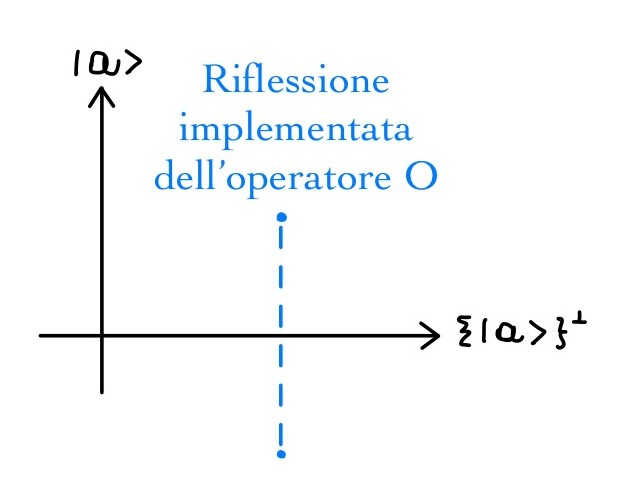
\includegraphics[scale=.45,keepaspectratio]{images/azioni_OG_1}} \quad
	\subfloat[][\label{subfig:azioni_OG_2} ]{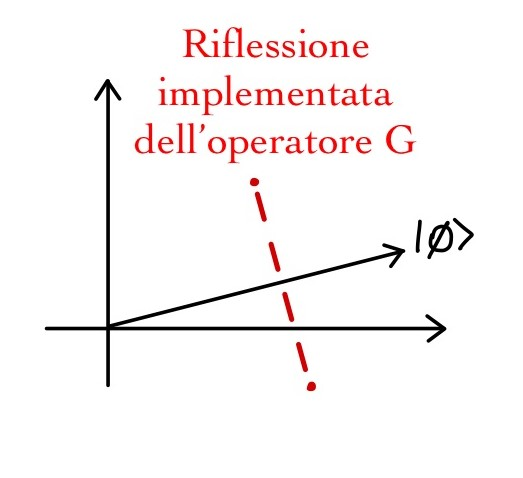
\includegraphics[scale=.45,keepaspectratio]{images/azioni_OG_2}} 
	\caption{\eqref{subfig:azioni_OG_1} L'operatore $O$ effettua una riflessione rispetto all'asse individuato da tutti gli stati perpendicolari ad $\ket{a}$. \eqref{subfig:azioni_OG_2} L'operatore $G$, invece, effettua una riflessione rispetto all'asse individuato dalla sovrapposizione di stati che abbiamo chiamato $\ket{\phi}$.}
\label{fig:azioni_OG}
\end{figure}
In termini matematici possiamo definire $O$ come
\begin{equation}\label{operator_O}
    O=\mathbb{I}-2\op{a}{a} \, ,
\end{equation}
infatti
\begin{align*}
    O\ket a &= \ket a -2\ket{a}\underbrace{\ip{a}{a}}_{1}= \ket a - 2\ket{a} = -\ket{a} \, , &\text{ per } \ket{x} &= \ket{a} \, , \\
    O\ket x &= \ket x -2\ket{a}\underbrace{\ip{a}{x}}_{0}= \ket{x} \, , &\text{ per } \ket{x} &\in \{ \ket{a} \}^\perp \, .
\end{align*}
Chiamiamo lo stato finale del data register nel modo seguente 
\begin{equation}\label{sovrapposizione_phi}
    \ket{0}^{\otimes n}\rightarrow H^{\otimes n}\ket{0}^{\otimes n}=\frac{1}{2^{\frac n2}}\sum_{x=0}^{2^n-1} \ket{x} \equiv \ket\phi \, ;
\end{equation}
notiamo che si tratta di una sovrapposizione uniforme di tutti i possibili interi con la stessa ampiezza data da $1/2^{\frac{n}{2}}$. Definiamo ora un'altra operazione di riflessione, che chiamiamo $G$, rispetto a $\ket\phi$ tale per cui
\begin{equation*}
    \begin{cases}
        G\ket\phi=\ket\phi \, , &\text{ per }\ket{x} = \ket{\phi} \\
        G\ket x=-\ket x \, , &\text{ per } \ip{x}{\phi} = 0
    \end{cases} \, .
\end{equation*}
Si veda la Figura \ref{subfig:azioni_OG_2} per una semplice rappresentazione grafica. In questo modo vediamo che $G$ è simile alla forma della \eqref{operator_O}, ma con un segno invertito:
\begin{equation}\label{operator_G}
    G=2\op{\phi}{\phi}-\mathbb{I} \, .
\end{equation}
Consideriamo ora l'operazione seguente:
\begin{equation}\label{operatore_incognito}
    \begin{cases}
        \ket{0}^{\otimes n} \rightarrow \ket{0}^{\otimes n} \,  & \\
        \ket{x} \rightarrow -\ket{x} \, , & x  \neq 0
    \end{cases} \, ,
\end{equation}
il quale mantiene il "ground state" inalterato e inverte qualsiasi altro stato della base computazionale. Se supponiamo di poter trovare un circuito che implementi l'operazione precedente, allora l'operatore $G$ può essere costruito in termini di gate nel seguente modo
\begin{center}
    \mbox{
        \Qcircuit @C=1em @R=1em {
            & \qw                         & \multigate{2}{G} & \qw                     & \qw \\
            & \raisebox{.3em}{\vdots}     & \nghost{G}       & \raisebox{.3em}{\vdots} &     \\
            & \qw                         & \ghost{G}        & \qw                     & \qw
        }
    }
    \raisebox{-2.3em}{=}
    \mbox{
        \Qcircuit @C=1em @R=1em {
            & \qw
            & \multigate{2}{H^{\otimes n}}
            & \qw
            & \multigate{2}{
                \begin{array}{ll}
                    \ket{0}^{\otimes n} \rightarrow \ket{0}^{\otimes n} \\
                    \ket{x}^{\otimes n} \rightarrow -\ket{x}^{\otimes n}
                \end{array}}
            & \qw
            & \multigate{2}{H^{\otimes n}}
            & \qw
            & \qw 
            \\
            & \raisebox{.3em}{\vdots}
            & \nghost{H^{\otimes n}}
            & \raisebox{.3em}{\vdots}
            & \nghost{
                \begin{array}{cc}
                    \ket{0}^{\otimes n}\rightarrow \ket{0}^{\otimes n}\\
                    \ket{x}^{\otimes n}\rightarrow -\ket{x}^{\otimes n}
                \end{array}}
            & \raisebox{.3em}{\vdots}
            & \nghost{H^{\otimes n}}
            & \raisebox{.3em}{\vdots}
            &
            \\
            & \qw
            & \ghost{H^{\otimes n}}
            & \qw
            & \ghost{
                \begin{array}{ll}
                    \ket{0}^{\otimes n}\rightarrow \ket{0}^{\otimes n}\\
                    \ket{x}^{\otimes n}\rightarrow -\ket{x}^{\otimes n}
                \end{array}}
            & \qw
            & \ghost{H^{\otimes n}}
            & \qw
            & \qw
        }
    }
\end{center}
Notiamo che il circuito precedente riproduce la \eqref{operator_G}: ricordando infatti che $H^2 = \mathbb{I}$ (\texttt{H-gate} è unitario) e $\ket{\phi} \equiv H^{\otimes n} \ket{0}^{\otimes n}$ avremo
\begin{equation*}
    G = H^{\otimes n} \left( 2\ket{0}^{\otimes n}\bra{0}^{\otimes n}-\mathbb{I} \right) H^{\otimes n}=2\op{\phi}{\phi}-\mathbb{I} \, .
\end{equation*}
Abbiamo quindi le due operazioni $O$ e $G$ di Figura \ref{fig:azioni_OG}. L'idea alla base dell'algoritmo di Grover è l'applicazione ripetuta della successione di operazioni $O$ e $G$: dimostreremo tra un attimo che se applichiamo la successione $\ldots GOGOG \ldots OGOGO$ (termina con $O$, quindi $O$ è il primo operatore che viene applicato) costituita da $k$ volte l'applicazione di tali operazioni allora per $k = \order{\sqrt{N}}$ la probabilità che lo stato finale rimanente sia $\ket{a}$ è prossima ad 1. 

\noindent Vediamo due semplici modi per descrivere questo procedimento. 

\subsection{Interpretazione geometrica}
Vediamo il motivo della conclusione precedente secondo un semplice argomento geometrico. Il vettore $\ket{a}$ è un particolare stato della sovrapposizione \eqref{sovrapposizione_phi}, quindi possiamo chiedere di calcolare il seguente prodotto scalare:
\begin{equation*}
    \ip{a}{\phi}=\frac{1}{2^{\frac n2}} \ll 1 \, ;
\end{equation*}
il risultato è un numero molto piccolo perché stiamo assumendo che $n$ sia molto grande (come detto all'inizio, un algoritmo di ricerca è sensato solamente se il database contiene un numero enorme di oggetti). Questo significa che $\ket{\phi}$ è quasi ortogonale ad $\ket{a}$, ossia coincide quasi con l'asse orizzontale (si pensi alla Figura \ref{subfig:azioni_OG_2}). Si noti dalla Figura \ref{subfig:geometrico_1} che 
\begin{equation*}
    \sin \theta = \cos \! \left( \frac{\pi}{2} - \theta \right) = \ip{a}{\phi} = \frac{1}{2^{\frac{n}{2}}} \ll 1 \, , \quad \Rightarrow \quad \sin \theta \approx \theta = \frac{1}{2^{\frac{n}{2}}} \, .
\end{equation*}
Siccome i nostri oggetti nel database sono $N=2^n$ (con $N$ grande e $n$ numero di qubit), allora $\theta\sim 1/\sqrt{N}$. Cosa succede a $\ket{\phi}$ quando si applica la sequenza di $G$ ed $O$? Si veda l'esempio di Figura \ref{subfig:geometrico_2}: il primo step è $O$, ossia una riflessione lungo $\{ \ket{a} \}^\perp$, quindi $\ket{\phi}$ viene ribaltato al di sotto dell'asse orizzontale di un angolo $\theta$; lo step successivo è $G$, ossia una riflessione lungo $\ket{\phi}$, che riporta il vettore nel primo quadrante con un angolo $2 \theta$ da $\ket{\phi}$. Si noti che l'azione complessiva di $O$ e $G$ è una doppia riflessione, cioè una rotazione, per cui lo stato $\phi$ è passato da un angolo $\theta$ a un angolo $3\theta$ dall'asse orizzontale. Applicando, nei due step successivi, nuovamente la sequenza $GO$ (prima $O$ poi $G$) si passerà da un angolo $3\theta$ a $5\theta$. Iterando questo procedimento per $r$ iterazioni, avremo che l'angolo finale diventa $\theta +2r\theta$. Dopo quante iterazioni il vettore risulta essenzialmente verticale? In termine di angoli significa imporre che $\theta +2r\theta \simeq \frac{\pi}{2}$, quindi  $r \simeq \frac{\pi}{4\theta}-\frac 12$. Ma $\theta$ è piccolo, per cui il secondo termine è trascurabile e si ottiene 
\begin{equation*}
    r\approx \frac{\pi}{4\theta}=\frac \pi 4 \theta^{-1}\approx \frac \pi 4 \sqrt N \, ;
\end{equation*}
\begin{figure}[!b]
	\centering	
	\subfloat[][\label{subfig:geometrico_1} ]{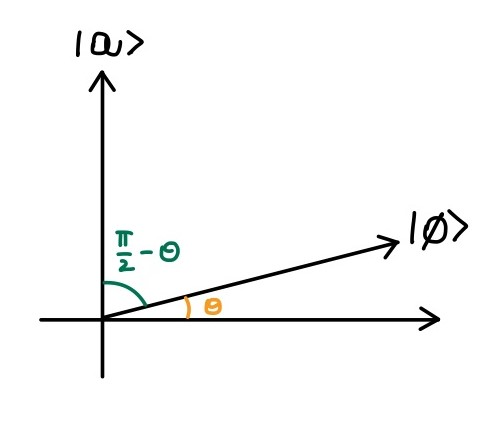
\includegraphics[scale=.4,keepaspectratio]{images/geometrico_1}} \quad
	\subfloat[][\label{subfig:geometrico_2} ]{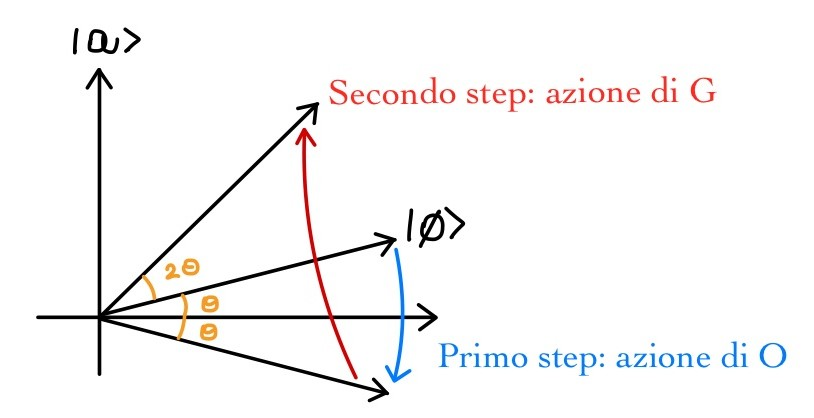
\includegraphics[scale=.4,keepaspectratio]{images/geometrico_2}} 
	\caption{\eqref{subfig:geometrico_1} Il prodotto scalare tra $\ket{a}$ e $\ket{\phi}$ è dato da $\cos \! \left( \frac{\pi}{2} - \theta \right) = \sin \theta$. \eqref{subfig:geometrico_2} Implementazione dei primi due step $GO$. Si noti che le due riflessioni corrispondono ad una rotazione: lo stato finale $GO \ket{\phi}$ è ruotato di angolo $2\theta$ rispetto a $\ket{\phi}$ e di angolo $3\theta$ rispetto all'asse orizzontale.}
\label{fig:geometrico}
\end{figure}
quindi dopo $\order{\sqrt N}$ iterazioni di $GO$ si arriva allo stato $\ket a$ con probabilità prossima ad 1: possiamo infatti trovare $\ket a$ attraverso una misura finale dello stato $(GO)^r\ket \phi$; si dimostra che  
\begin{equation*}
    (GO)^r\ket \phi = \sqrt{1-\varepsilon^2}\ket a + \varepsilon \ket{a}^\perp \, , \quad \varepsilon \ll 1 \, .
\end{equation*}
Se siamo sfortunati e non otteniamo $\ket a$, possiamo eseguire nuovamente l'algoritmo magari incrementando il numero di iterazioni e provare a misurare nuovamente. Dopo un numero limitato di tentativi troveremo $a$!


\subsection{Interpretazione grafica: inversione rispetto alla media}
Esiste un altro modo grafico per visualizzare il risultato dell'algoritmo di Grover. Supponiamo di partire con un generico stato $\ket \psi = \sum_x \alpha_x \ket x$ espanso nella base computazionale. Scriviamo esplicitamente l'azione di $O$ e $G$ su $\ket{\psi}$:
\begin{itemize}
    \item L'operatore $O$ è la riflessione rispetto alla direzione individuata da $\{ \ket{a} \}^\perp$, quindi inverte l'ampiezza solamente per $x=a$:
    \begin{equation*}
        O \, : \;
        \begin{cases}
            \alpha_a \rightarrow -\alpha_a \, , &x=a\\
            \alpha_x \rightarrow \alpha_x \, , &x\neq a
        \end{cases} \, .
    \end{equation*}
    
    \item Per capire l'azione di $G$, invece, ricordiamo la \eqref{operator_G} dove $\ket{\phi} = \frac{1}{2^{n/2}} \sum_x \ket{x} = \frac{1}{\sqrt{N}} \sum_x \ket{x}$. Calcoliamo $G \ket{\psi}$:
    \begin{align*}
        G \ket{\psi} &= \left( 2 \op{\phi} - \mathbb{I} \right) \ket{\psi} = \frac{2}{N} \sum_{x=0}^{2^n-1} \ket{x} \sum_{y=0}^{2^n-1} \bra{y} \left( \sum_{z=0}^{2^n-1} \alpha_z \ket{z} \right) - \sum_{x=0}^{2^n-1} \alpha_x \ket{x} \\
        &= \sum_{x=0}^{2^n-1} \left( 2 \sum_{y=0}^{2^n-1} \frac{\alpha_y}{N} - \alpha_x \right) \ket{x} \, ,
    \end{align*}
    dove a secondo passaggio abbiamo utilizzato $\braket{y}{z} = \delta_{yz}$ (si ricordi l'ortonormalizzazione degli stati della base computazionale). Perciò l'azione dell'operatore $G$ non è altro che una riflessione rispetto al valor medio dell'ampiezza:
    \begin{equation*}
        G \, : \; \alpha_x \rightarrow 2 \expval{\alpha} - \alpha_x \, , \; \text{ dove } \expval{\alpha} \equiv \sum_{y=0}^{2^n-1} \frac{\alpha_y}{N} \, .
    \end{equation*}
\end{itemize}
Ricordiamo che nell'algoritmo si parte dallo stato $\ket{\phi} = \frac{1}{\sqrt{N}} \sum_x \ket{x}$. Disegnando in ascissa i diversi stati e in ordinata l'ampiezza di ciascun stato, l'azione grafica ripetuta degli operatori $O$ e $G$ su $\ket{\phi}$ è mostrata nei diversi plot di Figura \ref{fig:plot_Grover}. È evidente come la continua applicazione di $O$ e $G$ ad ogni step faccia in modo che l'ampiezza di $\ket{a}$ aumenti sempre di più fino a 1 e le ampiezze degli stati rimanenti diminuiscano sempre di più tendendo a 0. 

\noindent Questo modo di procedere per visualizzare l'azione dell'algoritmo di Glover è utile anche nel caso in cui si voglia effettuare una ricerca di $M$ numeri speciali all'interno degli $N$ oggetti del database. Come evidenziano i plot di Figura \ref{fig:2_special_Grover}, dopo un certo numero di applicazioni di $O$ e $G$, le $M$ ampiezze cercate tendono al valore $1/M$ e si isolano automaticamente rispetto a tutte le altre.

\begin{figure}[!ht]
	\centering	
	\subfloat[][\text{Stato iniziale} $\ket{\phi}$.\label{subfig:plot_Grover_1} ]{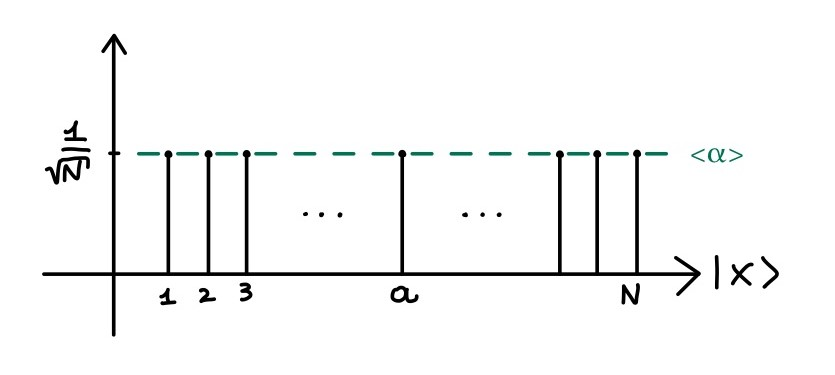
\includegraphics[scale=.35,keepaspectratio]{images/plot_Grover_1}} \quad
	\subfloat[][\text{Azione di }$O$: stato $O \ket{\phi}$.\label{subfig:plot_Grover_2} ]{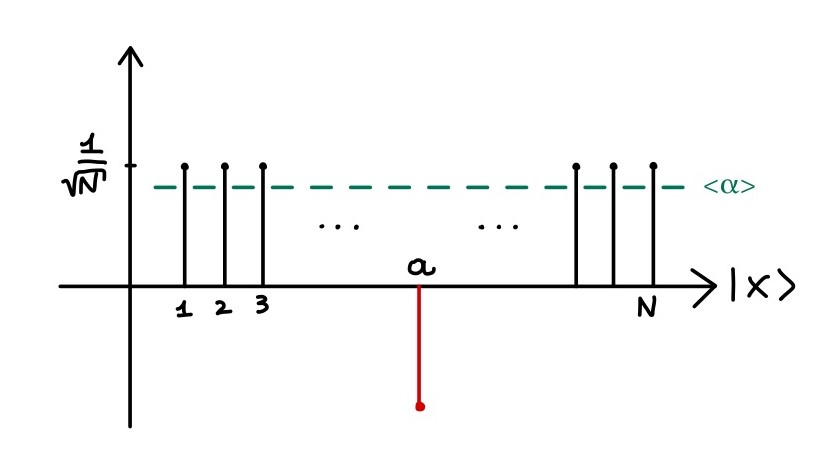
\includegraphics[scale=.35,keepaspectratio]{images/plot_Grover_2}} \\
	\subfloat[][\text{Azione di }$G$: stato $G O \ket{\phi}$.\label{subfig:plot_Grover_3} ]{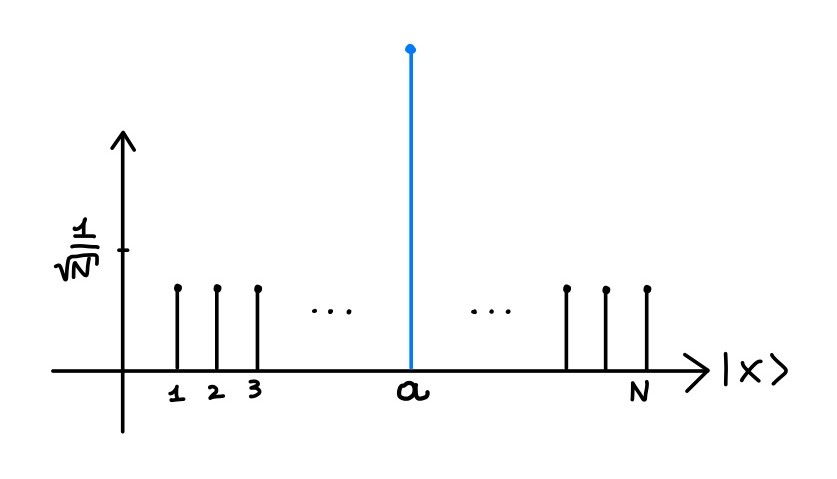
\includegraphics[scale=.35,keepaspectratio]{images/plot_Grover_3}} \\
	\subfloat[][\text{Azione di }$O$: stato $OGO \ket{\phi}$.\label{subfig:plot_Grover_4} ]{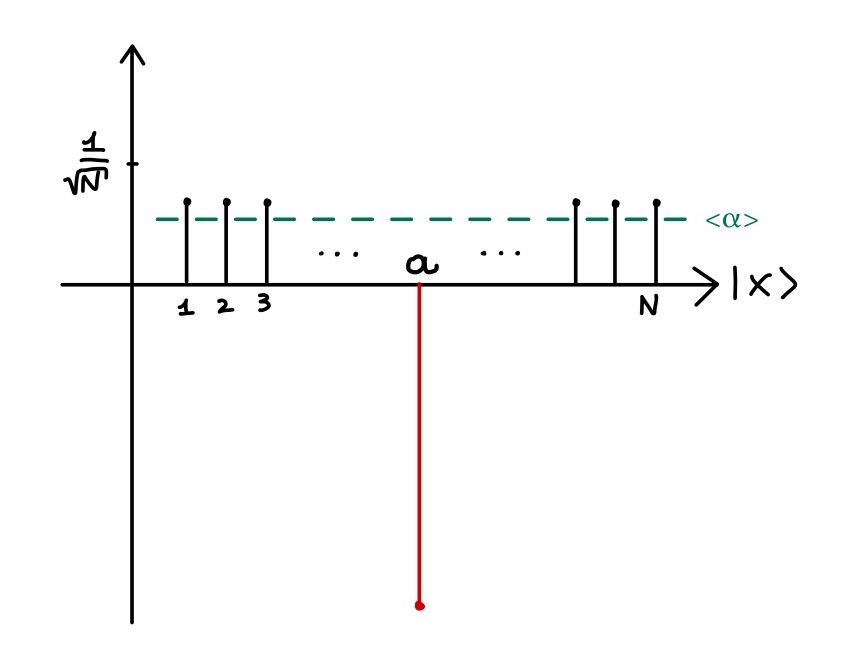
\includegraphics[scale=.35,keepaspectratio]{images/plot_Grover_4}} \quad
	\subfloat[][\text{Azione di }$G$: stato $GOGO \ket{\phi}$.\label{subfig:plot_Grover_5} ]{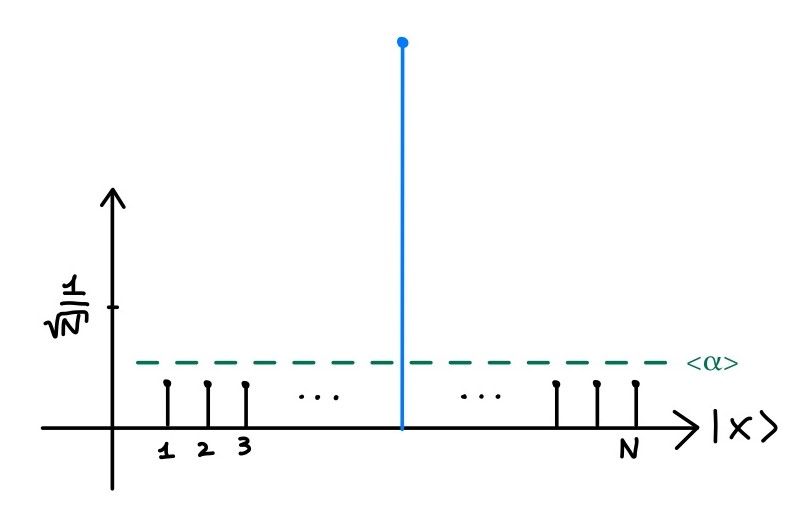
\includegraphics[scale=.35,keepaspectratio]{images/plot_Grover_5}} 
	\caption{Esempio dell'applicazione dei primi due step $GOGO$ allo stato $\ket{\phi}$. In rosso e in blu sono indicate le azioni di $O$ e $G$ rispettivamente sullo stato $\ket{a}$; in verde scuro (con una linea tratteggiata orizzontale) è mostrata la media $\expval{\alpha}$ delle ampiezze. Si noti come $O$ porti ogni volta ad una diminuzione della media (solo l'ampiezza di $\ket{a}$ è invertita); $G$, invece, causa una diminuzione di tutte le ampiezze di $\ket{x} \neq \ket{a}$ e un aumento dell'ampiezza di $\ket{a}$. Ad ogni step l'ampiezza di $\ket{a}$ diventa sempre più alta tendendo ad 1.}
\label{fig:plot_Grover}
\end{figure}

\begin{figure}[!ht]
	\centering	
	\subfloat[][\text{Configurazione iniziale}.\label{subfig:2_special_Grover_1} ]{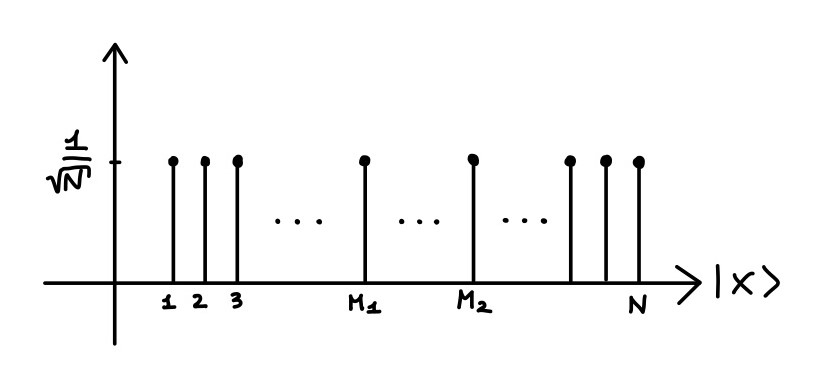
\includegraphics[scale=.35,keepaspectratio]{images/2_special_Grover_1}} \quad
	\subfloat[][\text{Azione di }$O$.\label{subfig:2_special_Grover_2} ]{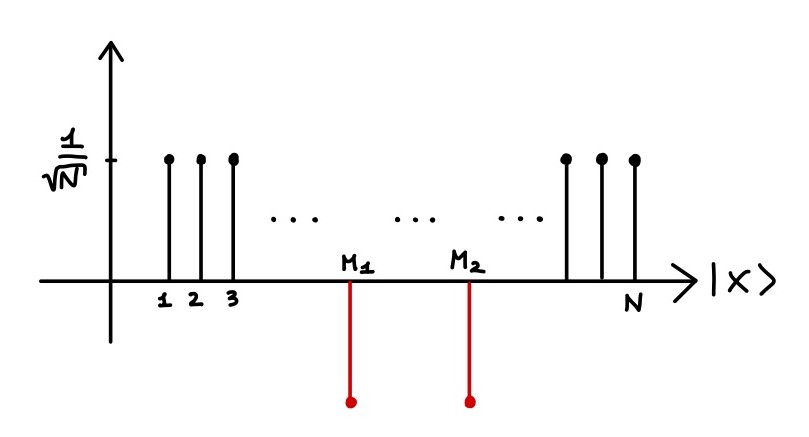
\includegraphics[scale=.35,keepaspectratio]{images/2_special_Grover_2}} \\
	\subfloat[][\text{Azione di }$G$.\label{subfig:2_special_Grover_3} ]{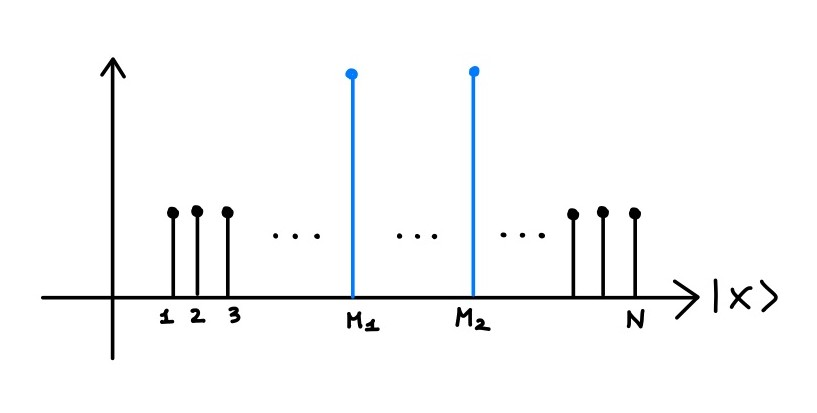
\includegraphics[scale=.35,keepaspectratio]{images/2_special_Grover_3}}
	\caption{Esempio di applicazione dell'algoritmo di ricerca di Grover per un database contenente due oggetti speciali, indicati con $M_1$ e $M_2$. In rosso e in blu sono mostrate le azioni di $O$ e $G$ sulle due ampiezze cercate.}
\label{fig:2_special_Grover}
\end{figure}

